\documentclass[1p]{elsarticle_modified}
%\bibliographystyle{elsarticle-num}

%\usepackage[colorlinks]{hyperref}
%\usepackage{abbrmath_seonhwa} %\Abb, \Ascr, \Acal ,\Abf, \Afrak
\usepackage{amsfonts}
\usepackage{amssymb}
\usepackage{amsmath}
\usepackage{amsthm}
\usepackage{scalefnt}
\usepackage{amsbsy}
\usepackage{kotex}
\usepackage{caption}
\usepackage{subfig}
\usepackage{color}
\usepackage{graphicx}
\usepackage{xcolor} %% white, black, red, green, blue, cyan, magenta, yellow
\usepackage{float}
\usepackage{setspace}
\usepackage{hyperref}

\usepackage{tikz}
\usetikzlibrary{arrows}

\usepackage{multirow}
\usepackage{array} % fixed length table
\usepackage{hhline}

%%%%%%%%%%%%%%%%%%%%%
\makeatletter
\renewcommand*\env@matrix[1][\arraystretch]{%
	\edef\arraystretch{#1}%
	\hskip -\arraycolsep
	\let\@ifnextchar\new@ifnextchar
	\array{*\c@MaxMatrixCols c}}
\makeatother %https://tex.stackexchange.com/questions/14071/how-can-i-increase-the-line-spacing-in-a-matrix
%%%%%%%%%%%%%%%

\usepackage[normalem]{ulem}

\newcommand{\msout}[1]{\ifmmode\text{\sout{\ensuremath{#1}}}\else\sout{#1}\fi}
%SOURCE: \msout is \stkout macro in https://tex.stackexchange.com/questions/20609/strikeout-in-math-mode

\newcommand{\cancel}[1]{
	\ifmmode
	{\color{red}\msout{#1}}
	\else
	{\color{red}\sout{#1}}
	\fi
}

\newcommand{\add}[1]{
	{\color{blue}\uwave{#1}}
}

\newcommand{\replace}[2]{
	\ifmmode
	{\color{red}\msout{#1}}{\color{blue}\uwave{#2}}
	\else
	{\color{red}\sout{#1}}{\color{blue}\uwave{#2}}
	\fi
}

\newcommand{\Sol}{\mathcal{S}} %segment
\newcommand{\D}{D} %diagram
\newcommand{\A}{\mathcal{A}} %arc


%%%%%%%%%%%%%%%%%%%%%%%%%%%%%5 test

\def\sl{\operatorname{\textup{SL}}(2,\Cbb)}
\def\psl{\operatorname{\textup{PSL}}(2,\Cbb)}
\def\quan{\mkern 1mu \triangleright \mkern 1mu}

\theoremstyle{definition}
\newtheorem{thm}{Theorem}[section]
\newtheorem{prop}[thm]{Proposition}
\newtheorem{lem}[thm]{Lemma}
\newtheorem{ques}[thm]{Question}
\newtheorem{cor}[thm]{Corollary}
\newtheorem{defn}[thm]{Definition}
\newtheorem{exam}[thm]{Example}
\newtheorem{rmk}[thm]{Remark}
\newtheorem{alg}[thm]{Algorithm}

\newcommand{\I}{\sqrt{-1}}
\begin{document}

%\begin{frontmatter}
%
%\title{Boundary parabolic representations of knots up to 8 crossings}
%
%%% Group authors per affiliation:
%\author{Yunhi Cho} 
%\address{Department of Mathematics, University of Seoul, Seoul, Korea}
%\ead{yhcho@uos.ac.kr}
%
%
%\author{Seonhwa Kim} %\fnref{s_kim}}
%\address{Center for Geometry and Physics, Institute for Basic Science, Pohang, 37673, Korea}
%\ead{ryeona17@ibs.re.kr}
%
%\author{Hyuk Kim}
%\address{Department of Mathematical Sciences, Seoul National University, Seoul 08826, Korea}
%\ead{hyukkim@snu.ac.kr}
%
%\author{Seokbeom Yoon}
%\address{Department of Mathematical Sciences, Seoul National University, Seoul, 08826,  Korea}
%\ead{sbyoon15@snu.ac.kr}
%
%\begin{abstract}
%We find all boundary parabolic representation of knots up to 8 crossings.
%
%\end{abstract}
%\begin{keyword}
%    \MSC[2010] 57M25 
%\end{keyword}
%
%\end{frontmatter}

%\linenumbers
%\tableofcontents
%
\newcommand\colored[1]{\textcolor{white}{\rule[-0.35ex]{0.8em}{1.4ex}}\kern-0.8em\color{red} #1}%
%\newcommand\colored[1]{\textcolor{white}{ #1}\kern-2.17ex	\textcolor{white}{ #1}\kern-1.81ex	\textcolor{white}{ #1}\kern-2.15ex\color{red}#1	}

{\Large $\underline{12a_{0297}~(K12a_{0297})}$}

\setlength{\tabcolsep}{10pt}
\renewcommand{\arraystretch}{1.6}
\vspace{1cm}\begin{tabular}{m{100pt}>{\centering\arraybackslash}m{274pt}}
\multirow{5}{120pt}{
	\centering
	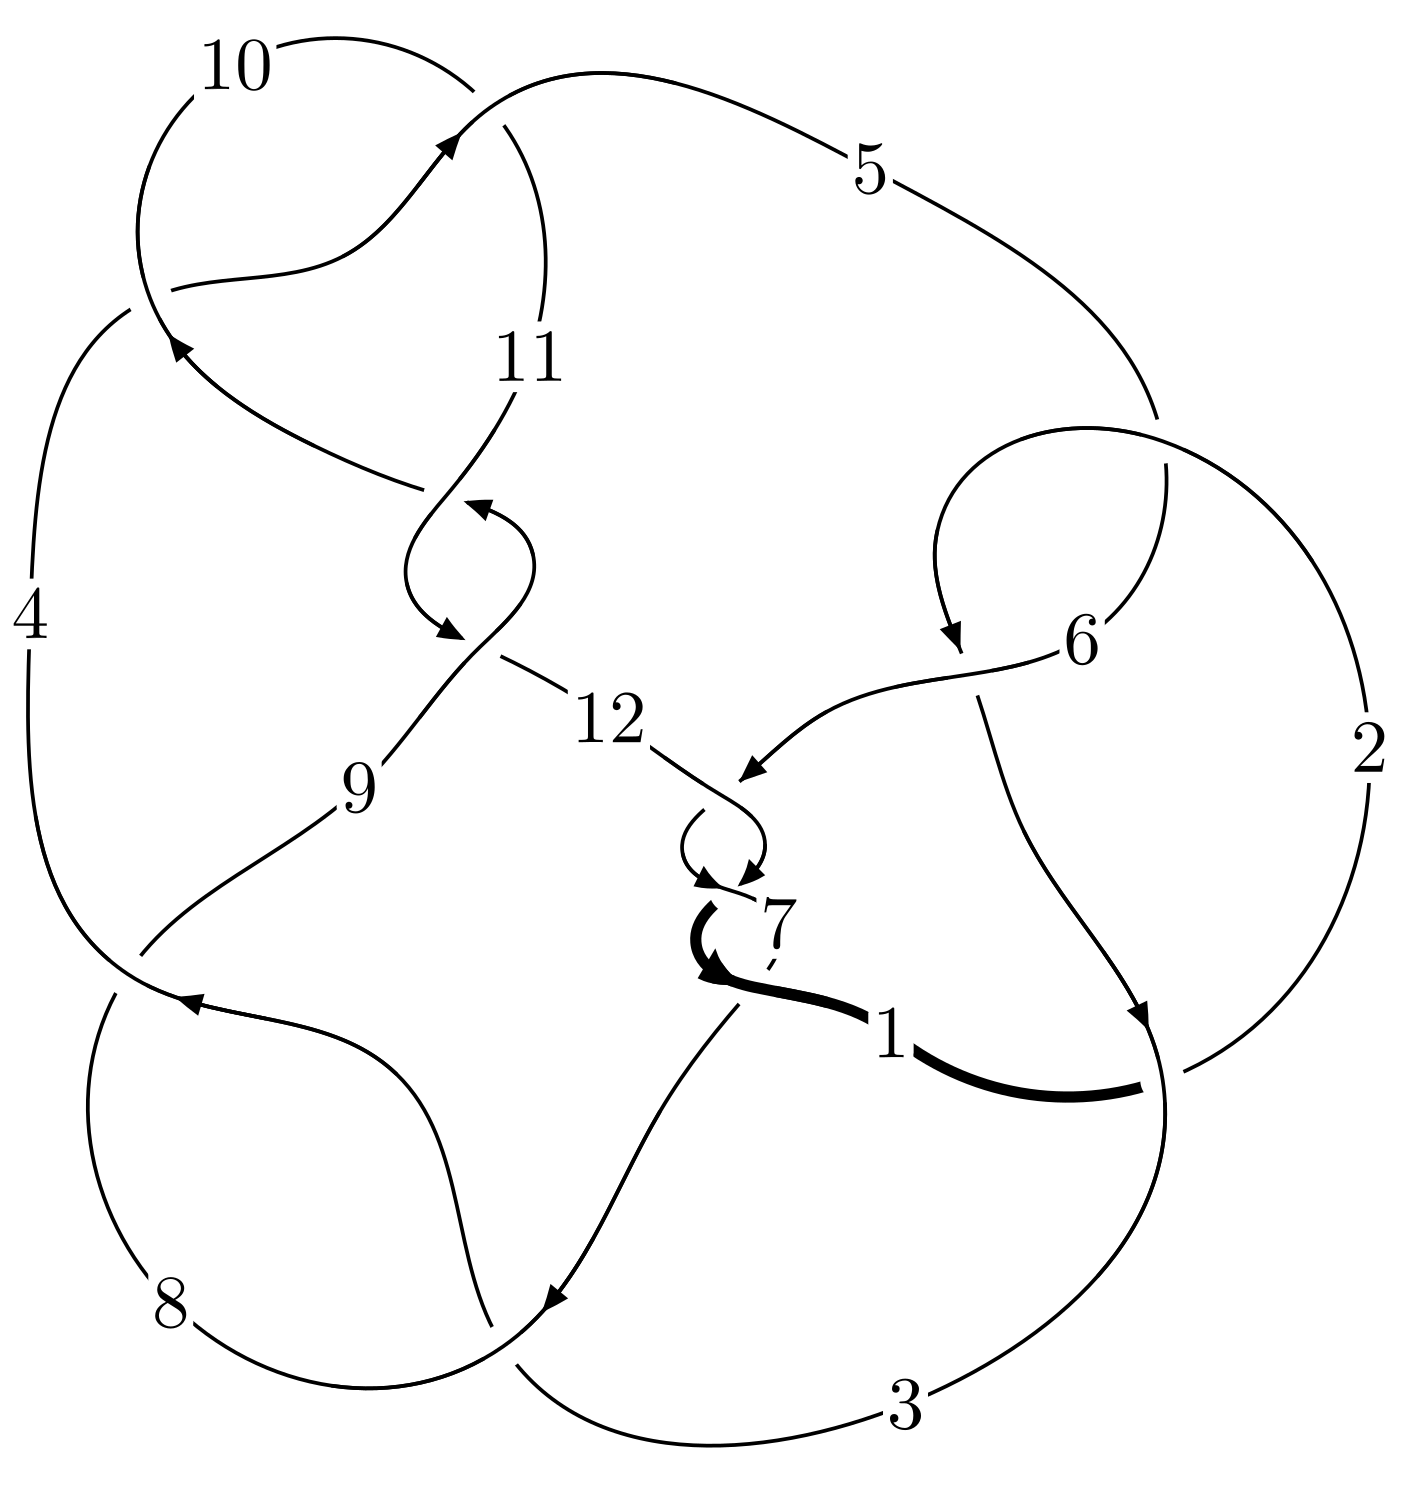
\includegraphics[width=112pt]{../../../GIT/diagram.site/Diagrams/png/1098_12a_0297.png}\\
\ \ \ A knot diagram\footnotemark}&
\allowdisplaybreaks
\textbf{Linearized knot diagam} \\
\cline{2-2}
 &
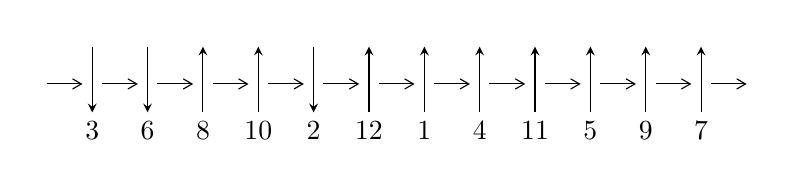
\begin{tikzpicture}[x=20pt, y=17pt]
	% nodes
	\node (C0) at (0, 0) {};
	\node (C1) at (1, 0) {};
	\node (C1U) at (1, +1) {};
	\node (C1D) at (1, -1) {3};

	\node (C2) at (2, 0) {};
	\node (C2U) at (2, +1) {};
	\node (C2D) at (2, -1) {6};

	\node (C3) at (3, 0) {};
	\node (C3U) at (3, +1) {};
	\node (C3D) at (3, -1) {8};

	\node (C4) at (4, 0) {};
	\node (C4U) at (4, +1) {};
	\node (C4D) at (4, -1) {10};

	\node (C5) at (5, 0) {};
	\node (C5U) at (5, +1) {};
	\node (C5D) at (5, -1) {2};

	\node (C6) at (6, 0) {};
	\node (C6U) at (6, +1) {};
	\node (C6D) at (6, -1) {12};

	\node (C7) at (7, 0) {};
	\node (C7U) at (7, +1) {};
	\node (C7D) at (7, -1) {1};

	\node (C8) at (8, 0) {};
	\node (C8U) at (8, +1) {};
	\node (C8D) at (8, -1) {4};

	\node (C9) at (9, 0) {};
	\node (C9U) at (9, +1) {};
	\node (C9D) at (9, -1) {11};

	\node (C10) at (10, 0) {};
	\node (C10U) at (10, +1) {};
	\node (C10D) at (10, -1) {5};

	\node (C11) at (11, 0) {};
	\node (C11U) at (11, +1) {};
	\node (C11D) at (11, -1) {9};

	\node (C12) at (12, 0) {};
	\node (C12U) at (12, +1) {};
	\node (C12D) at (12, -1) {7};
	\node (C13) at (13, 0) {};

	% arrows
	\draw[->,>={angle 60}]
	(C0) edge (C1) (C1) edge (C2) (C2) edge (C3) (C3) edge (C4) (C4) edge (C5) (C5) edge (C6) (C6) edge (C7) (C7) edge (C8) (C8) edge (C9) (C9) edge (C10) (C10) edge (C11) (C11) edge (C12) (C12) edge (C13) ;	\draw[->,>=stealth]
	(C1U) edge (C1D) (C2U) edge (C2D) (C3D) edge (C3U) (C4D) edge (C4U) (C5U) edge (C5D) (C6D) edge (C6U) (C7D) edge (C7U) (C8D) edge (C8U) (C9D) edge (C9U) (C10D) edge (C10U) (C11D) edge (C11U) (C12D) edge (C12U) ;
	\end{tikzpicture} \\
\hhline{~~} \\& 
\textbf{Solving Sequence} \\ \cline{2-2} 
 &
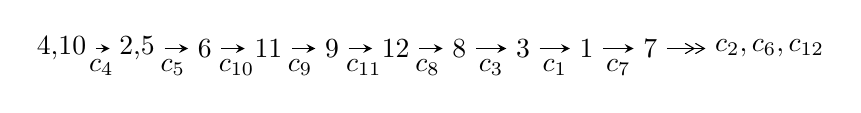
\begin{tikzpicture}[x=23pt, y=7pt]
	% node
	\node (A0) at (-1/8, 0) {4,10};
	\node (A1) at (17/16, 0) {2,5};
	\node (A2) at (17/8, 0) {6};
	\node (A3) at (25/8, 0) {11};
	\node (A4) at (33/8, 0) {9};
	\node (A5) at (41/8, 0) {12};
	\node (A6) at (49/8, 0) {8};
	\node (A7) at (57/8, 0) {3};
	\node (A8) at (65/8, 0) {1};
	\node (A9) at (73/8, 0) {7};
	\node (C1) at (1/2, -1) {$c_{4}$};
	\node (C2) at (13/8, -1) {$c_{5}$};
	\node (C3) at (21/8, -1) {$c_{10}$};
	\node (C4) at (29/8, -1) {$c_{9}$};
	\node (C5) at (37/8, -1) {$c_{11}$};
	\node (C6) at (45/8, -1) {$c_{8}$};
	\node (C7) at (53/8, -1) {$c_{3}$};
	\node (C8) at (61/8, -1) {$c_{1}$};
	\node (C9) at (69/8, -1) {$c_{7}$};
	\node (A10) at (11, 0) {$c_{2},c_{6},c_{12}$};

	% edge
	\draw[->,>=stealth]	
	(A0) edge (A1) (A1) edge (A2) (A2) edge (A3) (A3) edge (A4) (A4) edge (A5) (A5) edge (A6) (A6) edge (A7) (A7) edge (A8) (A8) edge (A9) ;
	\draw[->>,>={angle 60}]	
	(A9) edge (A10);
\end{tikzpicture} \\ 

\end{tabular} \\

\footnotetext{
The image of knot diagram is generated by the software ``\textbf{Draw programme}" developed by Andrew Bartholomew(\url{http://www.layer8.co.uk/maths/draw/index.htm\#Running-draw}), where we modified some parts for our purpose(\url{https://github.com/CATsTAILs/LinksPainter}).
}\phantom \\ \newline 
\centering \textbf{Ideals for irreducible components\footnotemark of $X_{\text{par}}$} 
 
\begin{align*}
I^u_{1}&=\langle 
2 u^{60}-3 u^{59}+\cdots+4 b-6,\;-2 u^{59}+19 u^{57}+\cdots+4 a-8,\;u^{61}-2 u^{60}+\cdots-4 u+2\rangle \\
I^u_{2}&=\langle 
-65 u^7 a^2+366 u^7 a+\cdots-730 a+714,\;2 u^7 a^2-4 u^7 a+\cdots+8 a-4,\\
\phantom{I^u_{2}}&\phantom{= \langle  }u^8+u^7- u^6-2 u^5+u^4+2 u^3-2 u-1\rangle \\
I^u_{3}&=\langle 
- u^2+b- u+1,\;- u^3+2 u^2+2 a+u,\;u^4- u^2+2\rangle \\
I^u_{4}&=\langle 
b-1,\;a+1,\;u-1\rangle \\
I^u_{5}&=\langle 
b-1,\;a,\;u+1\rangle \\
I^u_{6}&=\langle 
b+1,\;a-2,\;u-1\rangle \\
I^u_{7}&=\langle 
b,\;a-1,\;u+1\rangle \\
I^u_{8}&=\langle 
u^3+u^2+b+1,\;a- u-1,\;u^4+1\rangle \\
\\
I^v_{1}&=\langle 
a,\;b+1,\;v-1\rangle \\
\end{align*}
\raggedright * 9 irreducible components of $\dim_{\mathbb{C}}=0$, with total 98 representations.\\
\footnotetext{All coefficients of polynomials are rational numbers. But the coefficients are sometimes approximated in decimal forms when there is not enough margin.}
\newpage
\renewcommand{\arraystretch}{1}
\centering \section*{I. $I^u_{1}= \langle 2 u^{60}-3 u^{59}+\cdots+4 b-6,\;-2 u^{59}+19 u^{57}+\cdots+4 a-8,\;u^{61}-2 u^{60}+\cdots-4 u+2 \rangle$}
\flushleft \textbf{(i) Arc colorings}\\
\begin{tabular}{m{7pt} m{180pt} m{7pt} m{180pt} }
\flushright $a_{4}=$&$\begin{pmatrix}1\\0\end{pmatrix}$ \\
\flushright $a_{10}=$&$\begin{pmatrix}0\\u\end{pmatrix}$ \\
\flushright $a_{2}=$&$\begin{pmatrix}\frac{1}{2} u^{59}-\frac{19}{4} u^{57}+\cdots-\frac{3}{2} u+2\\-\frac{1}{2} u^{60}+\frac{3}{4} u^{59}+\cdots-\frac{5}{2} u+\frac{3}{2}\end{pmatrix}$ \\
\flushright $a_{5}=$&$\begin{pmatrix}1\\- u^2\end{pmatrix}$ \\
\flushright $a_{6}=$&$\begin{pmatrix}\frac{1}{2} u^{60}- u^{59}+\cdots-11 u^3-\frac{1}{2}\\u^{60}-10 u^{58}+\cdots+\frac{3}{2} u+1\end{pmatrix}$ \\
\flushright $a_{11}=$&$\begin{pmatrix}u\\- u^3+u\end{pmatrix}$ \\
\flushright $a_{9}=$&$\begin{pmatrix}- u^3\\u^5- u^3+u\end{pmatrix}$ \\
\flushright $a_{12}=$&$\begin{pmatrix}u^5+u\\- u^7+u^5-2 u^3+u\end{pmatrix}$ \\
\flushright $a_{8}=$&$\begin{pmatrix}- u^5- u\\u^5- u^3+u\end{pmatrix}$ \\
\flushright $a_{3}=$&$\begin{pmatrix}- u^{10}+u^8-2 u^6+u^4- u^2+1\\u^{10}-2 u^8+3 u^6-2 u^4+u^2\end{pmatrix}$ \\
\flushright $a_{1}=$&$\begin{pmatrix}\frac{1}{4} u^{56}-\frac{9}{4} u^{54}+\cdots-\frac{3}{2} u+\frac{1}{2}\\-\frac{1}{4} u^{58}+\frac{5}{2} u^{56}+\cdots+4 u^3- u\end{pmatrix}$ \\
\flushright $a_{7}=$&$\begin{pmatrix}\frac{1}{4} u^{56}-\frac{9}{4} u^{54}+\cdots-\frac{3}{2} u+\frac{1}{2}\\-\frac{1}{4} u^{56}+\frac{5}{2} u^{54}+\cdots-\frac{1}{2} u^2+u\end{pmatrix}$\\&\end{tabular}
\flushleft \textbf{(ii) Obstruction class $= -1$}\\~\\
\flushleft \textbf{(iii) Cusp Shapes $= 2 u^{60}-4 u^{59}+\cdots+16 u^2-2 u$}\\~\\
\newpage\renewcommand{\arraystretch}{1}
\flushleft \textbf{(iv) u-Polynomials at the component}\newline \\
\begin{tabular}{m{50pt}|m{274pt}}
Crossings & \hspace{64pt}u-Polynomials at each crossing \\
\hline $$\begin{aligned}c_{1}\end{aligned}$$&$\begin{aligned}
&u^{61}+21 u^{60}+\cdots+741 u+225
\end{aligned}$\\
\hline $$\begin{aligned}c_{2},c_{5}\end{aligned}$$&$\begin{aligned}
&u^{61}+3 u^{60}+\cdots+21 u-15
\end{aligned}$\\
\hline $$\begin{aligned}c_{3},c_{8}\end{aligned}$$&$\begin{aligned}
&u^{61}-2 u^{60}+\cdots-10164 u-3866
\end{aligned}$\\
\hline $$\begin{aligned}c_{4},c_{10}\end{aligned}$$&$\begin{aligned}
&u^{61}+2 u^{60}+\cdots-4 u-2
\end{aligned}$\\
\hline $$\begin{aligned}c_{6},c_{7},c_{12}\end{aligned}$$&$\begin{aligned}
&u^{61}-3 u^{60}+\cdots-15 u-17
\end{aligned}$\\
\hline $$\begin{aligned}c_{9},c_{11}\end{aligned}$$&$\begin{aligned}
&u^{61}-20 u^{60}+\cdots+44 u^2-4
\end{aligned}$\\
\hline
\end{tabular}\\~\\
\newpage\renewcommand{\arraystretch}{1}
\flushleft \textbf{(v) Riley Polynomials at the component}\newline \\
\begin{tabular}{m{50pt}|m{274pt}}
Crossings & \hspace{64pt}Riley Polynomials at each crossing \\
\hline $$\begin{aligned}c_{1}\end{aligned}$$&$\begin{aligned}
&y^{61}+51 y^{60}+\cdots-783819 y-50625
\end{aligned}$\\
\hline $$\begin{aligned}c_{2},c_{5}\end{aligned}$$&$\begin{aligned}
&y^{61}-21 y^{60}+\cdots+741 y-225
\end{aligned}$\\
\hline $$\begin{aligned}c_{3},c_{8}\end{aligned}$$&$\begin{aligned}
&y^{61}-44 y^{60}+\cdots+225348784 y-14945956
\end{aligned}$\\
\hline $$\begin{aligned}c_{4},c_{10}\end{aligned}$$&$\begin{aligned}
&y^{61}-20 y^{60}+\cdots+44 y^2-4
\end{aligned}$\\
\hline $$\begin{aligned}c_{6},c_{7},c_{12}\end{aligned}$$&$\begin{aligned}
&y^{61}-69 y^{60}+\cdots-14123 y-289
\end{aligned}$\\
\hline $$\begin{aligned}c_{9},c_{11}\end{aligned}$$&$\begin{aligned}
&y^{61}+40 y^{60}+\cdots+352 y-16
\end{aligned}$\\
\hline
\end{tabular}\\~\\
\newpage\flushleft \textbf{(vi) Complex Volumes and Cusp Shapes}
$$\begin{array}{c|c|c}  
\text{Solutions to }I^u_{1}& \I (\text{vol} + \sqrt{-1}CS) & \text{Cusp shape}\\
 \hline 
\begin{aligned}
u &= \phantom{-}0.684026 + 0.730349 I \\
a &= \phantom{-}1.009310 - 0.004276 I \\
b &= -0.980208 - 0.876387 I\end{aligned}
 & -3.51260 - 0.02973 I & -1.53347 - 0.41407 I \\ \hline\begin{aligned}
u &= \phantom{-}0.684026 - 0.730349 I \\
a &= \phantom{-}1.009310 + 0.004276 I \\
b &= -0.980208 + 0.876387 I\end{aligned}
 & -3.51260 + 0.02973 I & -1.53347 + 0.41407 I \\ \hline\begin{aligned}
u &= -0.596675 + 0.818364 I \\
a &= -0.780560 - 0.903959 I \\
b &= \phantom{-}1.80103 - 1.76065 I\end{aligned}
 & \phantom{-}5.86684 + 10.52580 I & \phantom{-}7.47241 - 5.20514 I \\ \hline\begin{aligned}
u &= -0.596675 - 0.818364 I \\
a &= -0.780560 + 0.903959 I \\
b &= \phantom{-}1.80103 + 1.76065 I\end{aligned}
 & \phantom{-}5.86684 - 10.52580 I & \phantom{-}7.47241 + 5.20514 I \\ \hline\begin{aligned}
u &= \phantom{-}0.980120 + 0.257609 I \\
a &= \phantom{-}1.103770 + 0.621483 I \\
b &= \phantom{-}0.089020 - 0.363650 I\end{aligned}
 & \phantom{-}6.96905 + 0.16982 I & \phantom{-}14.1748 - 0.9961 I \\ \hline\begin{aligned}
u &= \phantom{-}0.980120 - 0.257609 I \\
a &= \phantom{-}1.103770 - 0.621483 I \\
b &= \phantom{-}0.089020 + 0.363650 I\end{aligned}
 & \phantom{-}6.96905 - 0.16982 I & \phantom{-}14.1748 + 0.9961 I \\ \hline\begin{aligned}
u &= \phantom{-}0.570037 + 0.804645 I \\
a &= \phantom{-}0.113760 - 0.379871 I \\
b &= \phantom{-}0.174544 - 1.221640 I\end{aligned}
 & \phantom{-}7.95075 - 4.31712 I & \phantom{-}9.88882 + 1.03046 I \\ \hline\begin{aligned}
u &= \phantom{-}0.570037 - 0.804645 I \\
a &= \phantom{-}0.113760 + 0.379871 I \\
b &= \phantom{-}0.174544 + 1.221640 I\end{aligned}
 & \phantom{-}7.95075 + 4.31712 I & \phantom{-}9.88882 - 1.03046 I \\ \hline\begin{aligned}
u &= \phantom{-}0.594682 + 0.783135 I \\
a &= -0.477300 + 1.212940 I \\
b &= \phantom{-}2.02601 + 1.39309 I\end{aligned}
 & -0.22057 - 6.22999 I & \phantom{-}4.63185 + 5.17897 I \\ \hline\begin{aligned}
u &= \phantom{-}0.594682 - 0.783135 I \\
a &= -0.477300 - 1.212940 I \\
b &= \phantom{-}2.02601 - 1.39309 I\end{aligned}
 & -0.22057 + 6.22999 I & \phantom{-}4.63185 - 5.17897 I\\
 \hline 
 \end{array}$$\newpage$$\begin{array}{c|c|c}  
\text{Solutions to }I^u_{1}& \I (\text{vol} + \sqrt{-1}CS) & \text{Cusp shape}\\
 \hline 
\begin{aligned}
u &= -0.971831 + 0.354476 I \\
a &= -0.11982 + 1.97303 I \\
b &= -0.327701 - 0.963726 I\end{aligned}
 & \phantom{-}6.46298 - 5.79381 I & \phantom{-}12.8562 + 6.6036 I \\ \hline\begin{aligned}
u &= -0.971831 - 0.354476 I \\
a &= -0.11982 - 1.97303 I \\
b &= -0.327701 + 0.963726 I\end{aligned}
 & \phantom{-}6.46298 + 5.79381 I & \phantom{-}12.8562 - 6.6036 I \\ \hline\begin{aligned}
u &= -0.693342 + 0.628373 I \\
a &= \phantom{-}1.030350 - 0.373254 I \\
b &= \phantom{-}0.509008 + 0.609720 I\end{aligned}
 & \phantom{-}0.288787 + 0.262438 I & \phantom{-}10.25017 - 1.54244 I \\ \hline\begin{aligned}
u &= -0.693342 - 0.628373 I \\
a &= \phantom{-}1.030350 + 0.373254 I \\
b &= \phantom{-}0.509008 - 0.609720 I\end{aligned}
 & \phantom{-}0.288787 - 0.262438 I & \phantom{-}10.25017 + 1.54244 I \\ \hline\begin{aligned}
u &= -0.741367 + 0.781988 I \\
a &= \phantom{-}0.968528 + 0.095329 I \\
b &= -0.766103 + 0.579735 I\end{aligned}
 & \phantom{-}0.550417 - 1.022540 I & \phantom{-}7.58092 + 2.83590 I \\ \hline\begin{aligned}
u &= -0.741367 - 0.781988 I \\
a &= \phantom{-}0.968528 - 0.095329 I \\
b &= -0.766103 - 0.579735 I\end{aligned}
 & \phantom{-}0.550417 + 1.022540 I & \phantom{-}7.58092 - 2.83590 I \\ \hline\begin{aligned}
u &= -0.813495 + 0.728217 I \\
a &= \phantom{-}1.226460 - 0.093979 I \\
b &= -1.10886 + 1.83090 I\end{aligned}
 & -5.14522 + 0.66407 I & \phantom{-0.000000 } 0 \\ \hline\begin{aligned}
u &= -0.813495 - 0.728217 I \\
a &= \phantom{-}1.226460 + 0.093979 I \\
b &= -1.10886 - 1.83090 I\end{aligned}
 & -5.14522 - 0.66407 I & \phantom{-0.000000 } 0 \\ \hline\begin{aligned}
u &= -1.105450 + 0.040560 I \\
a &= -1.17835 - 2.39972 I \\
b &= \phantom{-}0.67943 + 2.15568 I\end{aligned}
 & \phantom{-}5.68265 - 5.26500 I & \phantom{-}11.79822 + 5.52257 I \\ \hline\begin{aligned}
u &= -1.105450 - 0.040560 I \\
a &= -1.17835 + 2.39972 I \\
b &= \phantom{-}0.67943 - 2.15568 I\end{aligned}
 & \phantom{-}5.68265 + 5.26500 I & \phantom{-}11.79822 - 5.52257 I\\
 \hline 
 \end{array}$$\newpage$$\begin{array}{c|c|c}  
\text{Solutions to }I^u_{1}& \I (\text{vol} + \sqrt{-1}CS) & \text{Cusp shape}\\
 \hline 
\begin{aligned}
u &= \phantom{-}0.798828 + 0.780694 I \\
a &= \phantom{-}1.072690 + 0.319738 I \\
b &= -0.61454 - 1.92988 I\end{aligned}
 & -0.34087 - 3.55037 I & \phantom{-}6.00000 + 0. I\phantom{ +0.000000I} \\ \hline\begin{aligned}
u &= \phantom{-}0.798828 - 0.780694 I \\
a &= \phantom{-}1.072690 - 0.319738 I \\
b &= -0.61454 + 1.92988 I\end{aligned}
 & -0.34087 + 3.55037 I & \phantom{-}6.00000 + 0. I\phantom{ +0.000000I} \\ \hline\begin{aligned}
u &= \phantom{-}0.456914 + 0.747552 I \\
a &= \phantom{-}0.187992 + 0.418041 I \\
b &= \phantom{-}0.929221 + 0.981503 I\end{aligned}
 & \phantom{-}8.62819 + 1.29175 I & \phantom{-}10.29853 - 0.71245 I \\ \hline\begin{aligned}
u &= \phantom{-}0.456914 - 0.747552 I \\
a &= \phantom{-}0.187992 - 0.418041 I \\
b &= \phantom{-}0.929221 - 0.981503 I\end{aligned}
 & \phantom{-}8.62819 - 1.29175 I & \phantom{-}10.29853 + 0.71245 I \\ \hline\begin{aligned}
u &= \phantom{-}1.128770 + 0.065228 I \\
a &= -0.96345 + 2.31373 I \\
b &= \phantom{-}0.41291 - 2.04529 I\end{aligned}
 & \phantom{-}12.1138 + 9.4985 I & \phantom{-}14.0807 - 5.6869 I \\ \hline\begin{aligned}
u &= \phantom{-}1.128770 - 0.065228 I \\
a &= -0.96345 - 2.31373 I \\
b &= \phantom{-}0.41291 + 2.04529 I\end{aligned}
 & \phantom{-}12.1138 - 9.4985 I & \phantom{-}14.0807 + 5.6869 I \\ \hline\begin{aligned}
u &= -1.133370 + 0.039127 I \\
a &= -1.07901 + 1.94352 I \\
b &= \phantom{-}0.67010 - 1.57030 I\end{aligned}
 & \phantom{-}13.9993 - 3.0917 I & \phantom{-}16.1356 + 0. I\phantom{ +0.000000I} \\ \hline\begin{aligned}
u &= -1.133370 - 0.039127 I \\
a &= -1.07901 - 1.94352 I \\
b &= \phantom{-}0.67010 + 1.57030 I\end{aligned}
 & \phantom{-}13.9993 + 3.0917 I & \phantom{-}16.1356 + 0. I\phantom{ +0.000000I} \\ \hline\begin{aligned}
u &= \phantom{-}0.789581 + 0.332833 I \\
a &= \phantom{-}0.29668 - 2.08794 I \\
b &= -0.413297 + 0.458976 I\end{aligned}
 & \phantom{-}0.18640 + 3.40430 I & \phantom{-}8.29784 - 8.43367 I \\ \hline\begin{aligned}
u &= \phantom{-}0.789581 - 0.332833 I \\
a &= \phantom{-}0.29668 + 2.08794 I \\
b &= -0.413297 - 0.458976 I\end{aligned}
 & \phantom{-}0.18640 - 3.40430 I & \phantom{-}8.29784 + 8.43367 I\\
 \hline 
 \end{array}$$\newpage$$\begin{array}{c|c|c}  
\text{Solutions to }I^u_{1}& \I (\text{vol} + \sqrt{-1}CS) & \text{Cusp shape}\\
 \hline 
\begin{aligned}
u &= -0.899967 + 0.713782 I \\
a &= -1.58036 + 1.59577 I \\
b &= -0.51410 - 2.10453 I\end{aligned}
 & -4.88256 - 6.15868 I & \phantom{-0.000000 } 0 \\ \hline\begin{aligned}
u &= -0.899967 - 0.713782 I \\
a &= -1.58036 - 1.59577 I \\
b &= -0.51410 + 2.10453 I\end{aligned}
 & -4.88256 + 6.15868 I & \phantom{-0.000000 } 0 \\ \hline\begin{aligned}
u &= -0.963966 + 0.649853 I \\
a &= -0.433033 - 0.566210 I \\
b &= \phantom{-}0.829635 - 0.624531 I\end{aligned}
 & \phantom{-}1.09575 - 5.31508 I & \phantom{-0.000000 } 0 \\ \hline\begin{aligned}
u &= -0.963966 - 0.649853 I \\
a &= -0.433033 + 0.566210 I \\
b &= \phantom{-}0.829635 + 0.624531 I\end{aligned}
 & \phantom{-}1.09575 + 5.31508 I & \phantom{-0.000000 } 0 \\ \hline\begin{aligned}
u &= -0.401857 + 0.728661 I \\
a &= -0.711645 + 1.063690 I \\
b &= \phantom{-}0.222763 + 0.716405 I\end{aligned}
 & \phantom{-}6.99087 - 7.50546 I & \phantom{-}8.25142 + 5.41277 I \\ \hline\begin{aligned}
u &= -0.401857 - 0.728661 I \\
a &= -0.711645 - 1.063690 I \\
b &= \phantom{-}0.222763 - 0.716405 I\end{aligned}
 & \phantom{-}6.99087 + 7.50546 I & \phantom{-}8.25142 - 5.41277 I \\ \hline\begin{aligned}
u &= \phantom{-}0.475808 + 0.672313 I \\
a &= -0.225590 - 1.386850 I \\
b &= -0.018272 - 0.781142 I\end{aligned}
 & \phantom{-}0.59272 + 3.70509 I & \phantom{-}5.79703 - 5.82804 I \\ \hline\begin{aligned}
u &= \phantom{-}0.475808 - 0.672313 I \\
a &= -0.225590 + 1.386850 I \\
b &= -0.018272 + 0.781142 I\end{aligned}
 & \phantom{-}0.59272 - 3.70509 I & \phantom{-}5.79703 + 5.82804 I \\ \hline\begin{aligned}
u &= \phantom{-}0.928616 + 0.747007 I \\
a &= -1.66826 - 1.18025 I \\
b &= -0.11509 + 2.08092 I\end{aligned}
 & \phantom{-}0.05447 + 9.30335 I & \phantom{-0.000000 } 0 \\ \hline\begin{aligned}
u &= \phantom{-}0.928616 - 0.747007 I \\
a &= -1.66826 + 1.18025 I \\
b &= -0.11509 - 2.08092 I\end{aligned}
 & \phantom{-}0.05447 - 9.30335 I & \phantom{-0.000000 } 0\\
 \hline 
 \end{array}$$\newpage$$\begin{array}{c|c|c}  
\text{Solutions to }I^u_{1}& \I (\text{vol} + \sqrt{-1}CS) & \text{Cusp shape}\\
 \hline 
\begin{aligned}
u &= \phantom{-}0.990835 + 0.679184 I \\
a &= -0.347057 - 1.318090 I \\
b &= -0.534238 + 1.253020 I\end{aligned}
 & -2.58879 + 5.43080 I & \phantom{-0.000000 } 0 \\ \hline\begin{aligned}
u &= \phantom{-}0.990835 - 0.679184 I \\
a &= -0.347057 + 1.318090 I \\
b &= -0.534238 - 1.253020 I\end{aligned}
 & -2.58879 - 5.43080 I & \phantom{-0.000000 } 0 \\ \hline\begin{aligned}
u &= \phantom{-}1.028240 + 0.622031 I \\
a &= -1.253520 - 0.573644 I \\
b &= -0.78894 + 1.32269 I\end{aligned}
 & \phantom{-}2.08349 + 1.29638 I & \phantom{-0.000000 } 0 \\ \hline\begin{aligned}
u &= \phantom{-}1.028240 - 0.622031 I \\
a &= -1.253520 + 0.573644 I \\
b &= -0.78894 - 1.32269 I\end{aligned}
 & \phantom{-}2.08349 - 1.29638 I & \phantom{-0.000000 } 0 \\ \hline\begin{aligned}
u &= -1.051030 + 0.593594 I \\
a &= -1.092970 + 0.306940 I \\
b &= -0.664632 - 0.819333 I\end{aligned}
 & \phantom{-}8.82075 + 2.55632 I & \phantom{-0.000000 } 0 \\ \hline\begin{aligned}
u &= -1.051030 - 0.593594 I \\
a &= -1.092970 - 0.306940 I \\
b &= -0.664632 + 0.819333 I\end{aligned}
 & \phantom{-}8.82075 - 2.55632 I & \phantom{-0.000000 } 0 \\ \hline\begin{aligned}
u &= -0.967643 + 0.722048 I \\
a &= -0.001148 + 0.746254 I \\
b &= -0.390854 - 0.853517 I\end{aligned}
 & \phantom{-}1.23996 - 4.65549 I & \phantom{-0.000000 } 0 \\ \hline\begin{aligned}
u &= -0.967643 - 0.722048 I \\
a &= -0.001148 - 0.746254 I \\
b &= -0.390854 + 0.853517 I\end{aligned}
 & \phantom{-}1.23996 + 4.65549 I & \phantom{-0.000000 } 0 \\ \hline\begin{aligned}
u &= \phantom{-}1.055860 + 0.618891 I \\
a &= \phantom{-}0.58117 + 1.82280 I \\
b &= \phantom{-}1.34616 - 1.10013 I\end{aligned}
 & \phantom{-}10.34380 + 3.85829 I & \phantom{-0.000000 } 0 \\ \hline\begin{aligned}
u &= \phantom{-}1.055860 - 0.618891 I \\
a &= \phantom{-}0.58117 - 1.82280 I \\
b &= \phantom{-}1.34616 + 1.10013 I\end{aligned}
 & \phantom{-}10.34380 - 3.85829 I & \phantom{-0.000000 } 0\\
 \hline 
 \end{array}$$\newpage$$\begin{array}{c|c|c}  
\text{Solutions to }I^u_{1}& \I (\text{vol} + \sqrt{-1}CS) & \text{Cusp shape}\\
 \hline 
\begin{aligned}
u &= \phantom{-}1.040000 + 0.677333 I \\
a &= \phantom{-}0.70242 + 2.72007 I \\
b &= \phantom{-}2.36433 - 2.02891 I\end{aligned}
 & \phantom{-}1.10337 + 11.75260 I & \phantom{-0.000000 } 0 \\ \hline\begin{aligned}
u &= \phantom{-}1.040000 - 0.677333 I \\
a &= \phantom{-}0.70242 - 2.72007 I \\
b &= \phantom{-}2.36433 + 2.02891 I\end{aligned}
 & \phantom{-}1.10337 - 11.75260 I & \phantom{-0.000000 } 0 \\ \hline\begin{aligned}
u &= \phantom{-}1.054830 + 0.675605 I \\
a &= -1.53601 - 0.38119 I \\
b &= -0.01333 + 1.41794 I\end{aligned}
 & \phantom{-}9.39588 + 9.88209 I & \phantom{-0.000000 } 0 \\ \hline\begin{aligned}
u &= \phantom{-}1.054830 - 0.675605 I \\
a &= -1.53601 + 0.38119 I \\
b &= -0.01333 - 1.41794 I\end{aligned}
 & \phantom{-}9.39588 - 9.88209 I & \phantom{-0.000000 } 0 \\ \hline\begin{aligned}
u &= -1.051510 + 0.689969 I \\
a &= \phantom{-}1.00404 - 2.59975 I \\
b &= \phantom{-}1.96259 + 2.37317 I\end{aligned}
 & \phantom{-}7.2336 - 16.1846 I & \phantom{-0.000000 } 0 \\ \hline\begin{aligned}
u &= -1.051510 - 0.689969 I \\
a &= \phantom{-}1.00404 + 2.59975 I \\
b &= \phantom{-}1.96259 - 2.37317 I\end{aligned}
 & \phantom{-}7.2336 + 16.1846 I & \phantom{-0.000000 } 0 \\ \hline\begin{aligned}
u &= -0.060491 + 0.608567 I \\
a &= \phantom{-}0.847236 - 0.127415 I \\
b &= -0.534181 + 0.678808 I\end{aligned}
 & \phantom{-}3.78928 + 2.56985 I & \phantom{-}6.99731 - 2.63136 I \\ \hline\begin{aligned}
u &= -0.060491 - 0.608567 I \\
a &= \phantom{-}0.847236 + 0.127415 I \\
b &= -0.534181 - 0.678808 I\end{aligned}
 & \phantom{-}3.78928 - 2.56985 I & \phantom{-}6.99731 + 2.63136 I \\ \hline\begin{aligned}
u &= -0.516262\phantom{ +0.000000I} \\
a &= \phantom{-}1.73864\phantom{ +0.000000I} \\
b &= \phantom{-}0.0487944\phantom{ +0.000000I}\end{aligned}
 & \phantom{-}0.822482\phantom{ +0.000000I} & \phantom{-}12.8010\phantom{ +0.000000I} \\ \hline\begin{aligned}
u &= \phantom{-}0.132981 + 0.413625 I \\
a &= \phantom{-}0.934359 + 0.065152 I \\
b &= -0.756818 - 0.341461 I\end{aligned}
 & -1.53288 - 0.93105 I & -1.52612 + 1.38760 I\\
 \hline 
 \end{array}$$\newpage$$\begin{array}{c|c|c}  
\text{Solutions to }I^u_{1}& \I (\text{vol} + \sqrt{-1}CS) & \text{Cusp shape}\\
 \hline 
\begin{aligned}
u &= \phantom{-}0.132981 - 0.413625 I \\
a &= \phantom{-}0.934359 - 0.065152 I \\
b &= -0.756818 + 0.341461 I\end{aligned}
 & -1.53288 + 0.93105 I & -1.52612 - 1.38760 I\\
 \hline 
 \end{array}$$\newpage\newpage\renewcommand{\arraystretch}{1}
\centering \section*{II. $I^u_{2}= \langle -65 u^7 a^2+366 u^7 a+\cdots-730 a+714,\;2 u^7 a^2-4 u^7 a+\cdots+8 a-4,\;u^8+u^7- u^6-2 u^5+u^4+2 u^3-2 u-1 \rangle$}
\flushleft \textbf{(i) Arc colorings}\\
\begin{tabular}{m{7pt} m{180pt} m{7pt} m{180pt} }
\flushright $a_{4}=$&$\begin{pmatrix}1\\0\end{pmatrix}$ \\
\flushright $a_{10}=$&$\begin{pmatrix}0\\u\end{pmatrix}$ \\
\flushright $a_{2}=$&$\begin{pmatrix}a\\0.631068 a^{2} u^{7}-3.55340 a u^{7}+\cdots+7.08738 a-6.93204\end{pmatrix}$ \\
\flushright $a_{5}=$&$\begin{pmatrix}1\\- u^2\end{pmatrix}$ \\
\flushright $a_{6}=$&$\begin{pmatrix}1.32039 a^{2} u^{7}-5.01942 a u^{7}+\cdots+9.21359 a-7.61165\\-1.66990 a^{2} u^{7}+5.49515 a u^{7}+\cdots-8.44660 a+8.09709\end{pmatrix}$ \\
\flushright $a_{11}=$&$\begin{pmatrix}u\\- u^3+u\end{pmatrix}$ \\
\flushright $a_{9}=$&$\begin{pmatrix}- u^3\\u^5- u^3+u\end{pmatrix}$ \\
\flushright $a_{12}=$&$\begin{pmatrix}u^5+u\\- u^7+u^5-2 u^3+u\end{pmatrix}$ \\
\flushright $a_{8}=$&$\begin{pmatrix}- u^5- u\\u^5- u^3+u\end{pmatrix}$ \\
\flushright $a_{3}=$&$\begin{pmatrix}- u^5- u\\u^7- u^5+2 u^3- u\end{pmatrix}$ \\
\flushright $a_{1}=$&$\begin{pmatrix}0.834951 a^{2} u^{7}-1.74757 a u^{7}+\cdots+4.22330 a-3.04854\\0.174757 a^{2} u^{7}-4.73786 a u^{7}+\cdots+8.11650 a-7.24272\end{pmatrix}$ \\
\flushright $a_{7}=$&$\begin{pmatrix}0.834951 a^{2} u^{7}-1.74757 a u^{7}+\cdots+4.22330 a-3.04854\\-0.776699 a^{2} u^{7}+4.83495 a u^{7}+\cdots-9.18447 a+9.30097\end{pmatrix}$\\&\end{tabular}
\flushleft \textbf{(ii) Obstruction class $= -1$}\\~\\
\flushleft \textbf{(iii) Cusp Shapes $= -4 u^7+8 u^5+4 u^4-8 u^3-4 u^2+4 u+14$}\\~\\
\newpage\renewcommand{\arraystretch}{1}
\flushleft \textbf{(iv) u-Polynomials at the component}\newline \\
\begin{tabular}{m{50pt}|m{274pt}}
Crossings & \hspace{64pt}u-Polynomials at each crossing \\
\hline $$\begin{aligned}c_{1}\end{aligned}$$&$\begin{aligned}
&u^{24}+16 u^{23}+\cdots+4 u+1
\end{aligned}$\\
\hline $$\begin{aligned}c_{2},c_{5},c_{6}\\c_{7},c_{12}\end{aligned}$$&$\begin{aligned}
&u^{24}-8 u^{22}+\cdots+2 u-1
\end{aligned}$\\
\hline $$\begin{aligned}c_{3},c_{8}\end{aligned}$$&$\begin{aligned}
&(u^8+u^7-3 u^6-2 u^5+3 u^4+2 u-1)^3
\end{aligned}$\\
\hline $$\begin{aligned}c_{4},c_{10}\end{aligned}$$&$\begin{aligned}
&(u^8- u^7- u^6+2 u^5+u^4-2 u^3+2 u-1)^3
\end{aligned}$\\
\hline $$\begin{aligned}c_{9},c_{11}\end{aligned}$$&$\begin{aligned}
&(u^8-3 u^7+7 u^6-10 u^5+11 u^4-10 u^3+6 u^2-4 u+1)^3
\end{aligned}$\\
\hline
\end{tabular}\\~\\
\newpage\renewcommand{\arraystretch}{1}
\flushleft \textbf{(v) Riley Polynomials at the component}\newline \\
\begin{tabular}{m{50pt}|m{274pt}}
Crossings & \hspace{64pt}Riley Polynomials at each crossing \\
\hline $$\begin{aligned}c_{1}\end{aligned}$$&$\begin{aligned}
&y^{24}-16 y^{23}+\cdots-12 y+1
\end{aligned}$\\
\hline $$\begin{aligned}c_{2},c_{5},c_{6}\\c_{7},c_{12}\end{aligned}$$&$\begin{aligned}
&y^{24}-16 y^{23}+\cdots-4 y+1
\end{aligned}$\\
\hline $$\begin{aligned}c_{3},c_{8}\end{aligned}$$&$\begin{aligned}
&(y^8-7 y^7+19 y^6-22 y^5+3 y^4+14 y^3-6 y^2-4 y+1)^3
\end{aligned}$\\
\hline $$\begin{aligned}c_{4},c_{10}\end{aligned}$$&$\begin{aligned}
&(y^8-3 y^7+7 y^6-10 y^5+11 y^4-10 y^3+6 y^2-4 y+1)^3
\end{aligned}$\\
\hline $$\begin{aligned}c_{9},c_{11}\end{aligned}$$&$\begin{aligned}
&(y^8+5 y^7+11 y^6+6 y^5-17 y^4-34 y^3-22 y^2-4 y+1)^3
\end{aligned}$\\
\hline
\end{tabular}\\~\\
\newpage\flushleft \textbf{(vi) Complex Volumes and Cusp Shapes}
$$\begin{array}{c|c|c}  
\text{Solutions to }I^u_{2}& \I (\text{vol} + \sqrt{-1}CS) & \text{Cusp shape}\\
 \hline 
\begin{aligned}
u &= -0.570868 + 0.730671 I \\
a &= \phantom{-}1.043500 - 0.060246 I \\
b &= -1.101120 + 0.799785 I\end{aligned}
 & \phantom{-}1.04066 + 1.13123 I & \phantom{-}7.41522 - 0.51079 I \\ \hline\begin{aligned}
u &= -0.570868 + 0.730671 I \\
a &= \phantom{-}0.359671 + 0.817635 I \\
b &= -0.016317 + 1.139980 I\end{aligned}
 & \phantom{-}1.04066 + 1.13123 I & \phantom{-}7.41522 - 0.51079 I \\ \hline\begin{aligned}
u &= -0.570868 + 0.730671 I \\
a &= \phantom{-}0.208103 - 1.124120 I \\
b &= \phantom{-}1.75850 - 0.67186 I\end{aligned}
 & \phantom{-}1.04066 + 1.13123 I & \phantom{-}7.41522 - 0.51079 I \\ \hline\begin{aligned}
u &= -0.570868 - 0.730671 I \\
a &= \phantom{-}1.043500 + 0.060246 I \\
b &= -1.101120 - 0.799785 I\end{aligned}
 & \phantom{-}1.04066 - 1.13123 I & \phantom{-}7.41522 + 0.51079 I \\ \hline\begin{aligned}
u &= -0.570868 - 0.730671 I \\
a &= \phantom{-}0.359671 - 0.817635 I \\
b &= -0.016317 - 1.139980 I\end{aligned}
 & \phantom{-}1.04066 - 1.13123 I & \phantom{-}7.41522 + 0.51079 I \\ \hline\begin{aligned}
u &= -0.570868 - 0.730671 I \\
a &= \phantom{-}0.208103 + 1.124120 I \\
b &= \phantom{-}1.75850 + 0.67186 I\end{aligned}
 & \phantom{-}1.04066 - 1.13123 I & \phantom{-}7.41522 + 0.51079 I \\ \hline\begin{aligned}
u &= \phantom{-}0.855237 + 0.665892 I \\
a &= \phantom{-}1.278090 - 0.370791 I \\
b &= -1.93181 - 1.61226 I\end{aligned}
 & -2.15941 + 2.57849 I & \phantom{-}4.27708 - 3.56796 I \\ \hline\begin{aligned}
u &= \phantom{-}0.855237 + 0.665892 I \\
a &= \phantom{-}0.504800 + 0.137739 I \\
b &= \phantom{-}0.0664349 - 0.0459194 I\end{aligned}
 & -2.15941 + 2.57849 I & \phantom{-}4.27708 - 3.56796 I \\ \hline\begin{aligned}
u &= \phantom{-}0.855237 + 0.665892 I \\
a &= -1.40393 - 2.38771 I \\
b &= -1.22880 + 1.98137 I\end{aligned}
 & -2.15941 + 2.57849 I & \phantom{-}4.27708 - 3.56796 I \\ \hline\begin{aligned}
u &= \phantom{-}0.855237 - 0.665892 I \\
a &= \phantom{-}1.278090 + 0.370791 I \\
b &= -1.93181 + 1.61226 I\end{aligned}
 & -2.15941 - 2.57849 I & \phantom{-}4.27708 + 3.56796 I\\
 \hline 
 \end{array}$$\newpage$$\begin{array}{c|c|c}  
\text{Solutions to }I^u_{2}& \I (\text{vol} + \sqrt{-1}CS) & \text{Cusp shape}\\
 \hline 
\begin{aligned}
u &= \phantom{-}0.855237 - 0.665892 I \\
a &= \phantom{-}0.504800 - 0.137739 I \\
b &= \phantom{-}0.0664349 + 0.0459194 I\end{aligned}
 & -2.15941 - 2.57849 I & \phantom{-}4.27708 + 3.56796 I \\ \hline\begin{aligned}
u &= \phantom{-}0.855237 - 0.665892 I \\
a &= -1.40393 + 2.38771 I \\
b &= -1.22880 - 1.98137 I\end{aligned}
 & -2.15941 - 2.57849 I & \phantom{-}4.27708 + 3.56796 I \\ \hline\begin{aligned}
u &= \phantom{-}1.09818\phantom{ +0.000000I} \\
a &= \phantom{-}1.32236\phantom{ +0.000000I} \\
b &= -0.189255\phantom{ +0.000000I}\end{aligned}
 & \phantom{-}6.50273\phantom{ +0.000000I} & \phantom{-}13.8640\phantom{ +0.000000I} \\ \hline\begin{aligned}
u &= \phantom{-}1.09818\phantom{ +0.000000I} \\
a &= -1.39057 + 2.07577 I \\
b &= \phantom{-}0.97427 - 1.80941 I\end{aligned}
 & \phantom{-}6.50273\phantom{ +0.000000I} & \phantom{-}13.8640\phantom{ +0.000000I} \\ \hline\begin{aligned}
u &= \phantom{-}1.09818\phantom{ +0.000000I} \\
a &= -1.39057 - 2.07577 I \\
b &= \phantom{-}0.97427 + 1.80941 I\end{aligned}
 & \phantom{-}6.50273\phantom{ +0.000000I} & \phantom{-}13.8640\phantom{ +0.000000I} \\ \hline\begin{aligned}
u &= -1.031810 + 0.655470 I \\
a &= -1.50786 + 0.47222 I \\
b &= -0.28319 - 1.61385 I\end{aligned}
 & \phantom{-}2.37968 - 6.44354 I & \phantom{-}9.42845 + 5.29417 I \\ \hline\begin{aligned}
u &= -1.031810 + 0.655470 I \\
a &= -0.13296 + 1.59682 I \\
b &= -0.67376 - 1.25902 I\end{aligned}
 & \phantom{-}2.37968 - 6.44354 I & \phantom{-}9.42845 + 5.29417 I \\ \hline\begin{aligned}
u &= -1.031810 + 0.655470 I \\
a &= \phantom{-}0.22313 - 2.40784 I \\
b &= \phantom{-}2.31545 + 1.17039 I\end{aligned}
 & \phantom{-}2.37968 - 6.44354 I & \phantom{-}9.42845 + 5.29417 I \\ \hline\begin{aligned}
u &= -1.031810 - 0.655470 I \\
a &= -1.50786 - 0.47222 I \\
b &= -0.28319 + 1.61385 I\end{aligned}
 & \phantom{-}2.37968 + 6.44354 I & \phantom{-}9.42845 - 5.29417 I \\ \hline\begin{aligned}
u &= -1.031810 - 0.655470 I \\
a &= -0.13296 - 1.59682 I \\
b &= -0.67376 + 1.25902 I\end{aligned}
 & \phantom{-}2.37968 + 6.44354 I & \phantom{-}9.42845 - 5.29417 I\\
 \hline 
 \end{array}$$\newpage$$\begin{array}{c|c|c}  
\text{Solutions to }I^u_{2}& \I (\text{vol} + \sqrt{-1}CS) & \text{Cusp shape}\\
 \hline 
\begin{aligned}
u &= -1.031810 - 0.655470 I \\
a &= \phantom{-}0.22313 + 2.40784 I \\
b &= \phantom{-}2.31545 - 1.17039 I\end{aligned}
 & \phantom{-}2.37968 + 6.44354 I & \phantom{-}9.42845 - 5.29417 I \\ \hline\begin{aligned}
u &= -0.603304\phantom{ +0.000000I} \\
a &= \phantom{-}1.26502\phantom{ +0.000000I} \\
b &= -1.64063\phantom{ +0.000000I}\end{aligned}
 & \phantom{-}0.845036\phantom{ +0.000000I} & \phantom{-}11.8940\phantom{ +0.000000I} \\ \hline\begin{aligned}
u &= -0.603304\phantom{ +0.000000I} \\
a &= \phantom{-}1.52434 + 0.84915 I \\
b &= \phantom{-}0.0352752 - 0.0977915 I\end{aligned}
 & \phantom{-}0.845036\phantom{ +0.000000I} & \phantom{-}11.8940\phantom{ +0.000000I} \\ \hline\begin{aligned}
u &= -0.603304\phantom{ +0.000000I} \\
a &= \phantom{-}1.52434 - 0.84915 I \\
b &= \phantom{-}0.0352752 + 0.0977915 I\end{aligned}
 & \phantom{-}0.845036\phantom{ +0.000000I} & \phantom{-}11.8940\phantom{ +0.000000I}\\
 \hline 
 \end{array}$$\newpage\newpage\renewcommand{\arraystretch}{1}
\centering \section*{III. $I^u_{3}= \langle - u^2+b- u+1,\;- u^3+2 u^2+2 a+u,\;u^4- u^2+2 \rangle$}
\flushleft \textbf{(i) Arc colorings}\\
\begin{tabular}{m{7pt} m{180pt} m{7pt} m{180pt} }
\flushright $a_{4}=$&$\begin{pmatrix}1\\0\end{pmatrix}$ \\
\flushright $a_{10}=$&$\begin{pmatrix}0\\u\end{pmatrix}$ \\
\flushright $a_{2}=$&$\begin{pmatrix}\frac{1}{2} u^3- u^2-\frac{1}{2} u\\u^2+u-1\end{pmatrix}$ \\
\flushright $a_{5}=$&$\begin{pmatrix}1\\- u^2\end{pmatrix}$ \\
\flushright $a_{6}=$&$\begin{pmatrix}\frac{1}{2} u^3- u^2-\frac{1}{2} u+1\\u-1\end{pmatrix}$ \\
\flushright $a_{11}=$&$\begin{pmatrix}u\\- u^3+u\end{pmatrix}$ \\
\flushright $a_{9}=$&$\begin{pmatrix}- u^3\\- u\end{pmatrix}$ \\
\flushright $a_{12}=$&$\begin{pmatrix}u^3- u\\u\end{pmatrix}$ \\
\flushright $a_{8}=$&$\begin{pmatrix}- u^3+u\\- u\end{pmatrix}$ \\
\flushright $a_{3}=$&$\begin{pmatrix}-1\\u^2\end{pmatrix}$ \\
\flushright $a_{1}=$&$\begin{pmatrix}\frac{1}{2} u^3- u^2-\frac{1}{2} u+1\\u-1\end{pmatrix}$ \\
\flushright $a_{7}=$&$\begin{pmatrix}-\frac{1}{2} u^3- u^2+\frac{1}{2} u+1\\-1\end{pmatrix}$\\&\end{tabular}
\flushleft \textbf{(ii) Obstruction class $= 1$}\\~\\
\flushleft \textbf{(iii) Cusp Shapes $= -4 u^2+8$}\\~\\
\newpage\renewcommand{\arraystretch}{1}
\flushleft \textbf{(iv) u-Polynomials at the component}\newline \\
\begin{tabular}{m{50pt}|m{274pt}}
Crossings & \hspace{64pt}u-Polynomials at each crossing \\
\hline $$\begin{aligned}c_{1},c_{5},c_{6}\\c_{7}\end{aligned}$$&$\begin{aligned}
&(u-1)^4
\end{aligned}$\\
\hline $$\begin{aligned}c_{2},c_{12}\end{aligned}$$&$\begin{aligned}
&(u+1)^4
\end{aligned}$\\
\hline $$\begin{aligned}c_{3},c_{4},c_{8}\\c_{10}\end{aligned}$$&$\begin{aligned}
&u^4- u^2+2
\end{aligned}$\\
\hline $$\begin{aligned}c_{9}\end{aligned}$$&$\begin{aligned}
&(u^2+u+2)^2
\end{aligned}$\\
\hline $$\begin{aligned}c_{11}\end{aligned}$$&$\begin{aligned}
&(u^2- u+2)^2
\end{aligned}$\\
\hline
\end{tabular}\\~\\
\newpage\renewcommand{\arraystretch}{1}
\flushleft \textbf{(v) Riley Polynomials at the component}\newline \\
\begin{tabular}{m{50pt}|m{274pt}}
Crossings & \hspace{64pt}Riley Polynomials at each crossing \\
\hline $$\begin{aligned}c_{1},c_{2},c_{5}\\c_{6},c_{7},c_{12}\end{aligned}$$&$\begin{aligned}
&(y-1)^4
\end{aligned}$\\
\hline $$\begin{aligned}c_{3},c_{4},c_{8}\\c_{10}\end{aligned}$$&$\begin{aligned}
&(y^2- y+2)^2
\end{aligned}$\\
\hline $$\begin{aligned}c_{9},c_{11}\end{aligned}$$&$\begin{aligned}
&(y^2+3 y+4)^2
\end{aligned}$\\
\hline
\end{tabular}\\~\\
\newpage\flushleft \textbf{(vi) Complex Volumes and Cusp Shapes}
$$\begin{array}{c|c|c}  
\text{Solutions to }I^u_{3}& \I (\text{vol} + \sqrt{-1}CS) & \text{Cusp shape}\\
 \hline 
\begin{aligned}
u &= \phantom{-}0.978318 + 0.676097 I \\
a &= -1.19178 - 0.84480 I \\
b &= \phantom{-}0.47832 + 1.99897 I\end{aligned}
 & -0.82247 + 5.33349 I & \phantom{-}6.00000 - 5.29150 I \\ \hline\begin{aligned}
u &= \phantom{-}0.978318 - 0.676097 I \\
a &= -1.19178 + 0.84480 I \\
b &= \phantom{-}0.47832 - 1.99897 I\end{aligned}
 & -0.82247 - 5.33349 I & \phantom{-}6.00000 + 5.29150 I \\ \hline\begin{aligned}
u &= -0.978318 + 0.676097 I \\
a &= \phantom{-}0.19178 + 1.80095 I \\
b &= -1.47832 - 0.64678 I\end{aligned}
 & -0.82247 - 5.33349 I & \phantom{-}6.00000 + 5.29150 I \\ \hline\begin{aligned}
u &= -0.978318 - 0.676097 I \\
a &= \phantom{-}0.19178 - 1.80095 I \\
b &= -1.47832 + 0.64678 I\end{aligned}
 & -0.82247 + 5.33349 I & \phantom{-}6.00000 - 5.29150 I\\
 \hline 
 \end{array}$$\newpage\newpage\renewcommand{\arraystretch}{1}
\centering \section*{IV. $I^u_{4}= \langle b-1,\;a+1,\;u-1 \rangle$}
\flushleft \textbf{(i) Arc colorings}\\
\begin{tabular}{m{7pt} m{180pt} m{7pt} m{180pt} }
\flushright $a_{4}=$&$\begin{pmatrix}1\\0\end{pmatrix}$ \\
\flushright $a_{10}=$&$\begin{pmatrix}0\\1\end{pmatrix}$ \\
\flushright $a_{2}=$&$\begin{pmatrix}-1\\1\end{pmatrix}$ \\
\flushright $a_{5}=$&$\begin{pmatrix}1\\-1\end{pmatrix}$ \\
\flushright $a_{6}=$&$\begin{pmatrix}1\\-1\end{pmatrix}$ \\
\flushright $a_{11}=$&$\begin{pmatrix}1\\0\end{pmatrix}$ \\
\flushright $a_{9}=$&$\begin{pmatrix}-1\\1\end{pmatrix}$ \\
\flushright $a_{12}=$&$\begin{pmatrix}2\\-1\end{pmatrix}$ \\
\flushright $a_{8}=$&$\begin{pmatrix}-2\\1\end{pmatrix}$ \\
\flushright $a_{3}=$&$\begin{pmatrix}-1\\1\end{pmatrix}$ \\
\flushright $a_{1}=$&$\begin{pmatrix}-1\\1\end{pmatrix}$ \\
\flushright $a_{7}=$&$\begin{pmatrix}-1\\0\end{pmatrix}$\\&\end{tabular}
\flushleft \textbf{(ii) Obstruction class $= -1$}\\~\\
\flushleft \textbf{(iii) Cusp Shapes $= 18$}\\~\\
\newpage\renewcommand{\arraystretch}{1}
\flushleft \textbf{(iv) u-Polynomials at the component}\newline \\
\begin{tabular}{m{50pt}|m{274pt}}
Crossings & \hspace{64pt}u-Polynomials at each crossing \\
\hline $$\begin{aligned}c_{1},c_{2},c_{5}\end{aligned}$$&$\begin{aligned}
&u
\end{aligned}$\\
\hline $$\begin{aligned}c_{3},c_{4},c_{6}\\c_{7},c_{8},c_{10}\\c_{12}\end{aligned}$$&$\begin{aligned}
&u+1
\end{aligned}$\\
\hline $$\begin{aligned}c_{9},c_{11}\end{aligned}$$&$\begin{aligned}
&u-1
\end{aligned}$\\
\hline
\end{tabular}\\~\\
\newpage\renewcommand{\arraystretch}{1}
\flushleft \textbf{(v) Riley Polynomials at the component}\newline \\
\begin{tabular}{m{50pt}|m{274pt}}
Crossings & \hspace{64pt}Riley Polynomials at each crossing \\
\hline $$\begin{aligned}c_{1},c_{2},c_{5}\end{aligned}$$&$\begin{aligned}
&y
\end{aligned}$\\
\hline $$\begin{aligned}c_{3},c_{4},c_{6}\\c_{7},c_{8},c_{9}\\c_{10},c_{11},c_{12}\end{aligned}$$&$\begin{aligned}
&y-1
\end{aligned}$\\
\hline
\end{tabular}\\~\\
\newpage\flushleft \textbf{(vi) Complex Volumes and Cusp Shapes}
$$\begin{array}{c|c|c}  
\text{Solutions to }I^u_{4}& \I (\text{vol} + \sqrt{-1}CS) & \text{Cusp shape}\\
 \hline 
\begin{aligned}
u &= \phantom{-}1.00000\phantom{ +0.000000I} \\
a &= -1.00000\phantom{ +0.000000I} \\
b &= \phantom{-}1.00000\phantom{ +0.000000I}\end{aligned}
 & \phantom{-}4.93480\phantom{ +0.000000I} & \phantom{-}18.0000\phantom{ +0.000000I}\\
 \hline 
 \end{array}$$\newpage\newpage\renewcommand{\arraystretch}{1}
\centering \section*{V. $I^u_{5}= \langle b-1,\;a,\;u+1 \rangle$}
\flushleft \textbf{(i) Arc colorings}\\
\begin{tabular}{m{7pt} m{180pt} m{7pt} m{180pt} }
\flushright $a_{4}=$&$\begin{pmatrix}1\\0\end{pmatrix}$ \\
\flushright $a_{10}=$&$\begin{pmatrix}0\\-1\end{pmatrix}$ \\
\flushright $a_{2}=$&$\begin{pmatrix}0\\1\end{pmatrix}$ \\
\flushright $a_{5}=$&$\begin{pmatrix}1\\-1\end{pmatrix}$ \\
\flushright $a_{6}=$&$\begin{pmatrix}1\\0\end{pmatrix}$ \\
\flushright $a_{11}=$&$\begin{pmatrix}-1\\0\end{pmatrix}$ \\
\flushright $a_{9}=$&$\begin{pmatrix}1\\-1\end{pmatrix}$ \\
\flushright $a_{12}=$&$\begin{pmatrix}-2\\1\end{pmatrix}$ \\
\flushright $a_{8}=$&$\begin{pmatrix}2\\-1\end{pmatrix}$ \\
\flushright $a_{3}=$&$\begin{pmatrix}-1\\1\end{pmatrix}$ \\
\flushright $a_{1}=$&$\begin{pmatrix}1\\0\end{pmatrix}$ \\
\flushright $a_{7}=$&$\begin{pmatrix}3\\-1\end{pmatrix}$\\&\end{tabular}
\flushleft \textbf{(ii) Obstruction class $= 1$}\\~\\
\flushleft \textbf{(iii) Cusp Shapes $= 12$}\\~\\
\newpage\renewcommand{\arraystretch}{1}
\flushleft \textbf{(iv) u-Polynomials at the component}\newline \\
\begin{tabular}{m{50pt}|m{274pt}}
Crossings & \hspace{64pt}u-Polynomials at each crossing \\
\hline $$\begin{aligned}c_{1},c_{5},c_{6}\\c_{7},c_{8},c_{10}\\c_{11}\end{aligned}$$&$\begin{aligned}
&u-1
\end{aligned}$\\
\hline $$\begin{aligned}c_{2},c_{3},c_{4}\\c_{9},c_{12}\end{aligned}$$&$\begin{aligned}
&u+1
\end{aligned}$\\
\hline
\end{tabular}\\~\\
\newpage\renewcommand{\arraystretch}{1}
\flushleft \textbf{(v) Riley Polynomials at the component}\newline \\
\begin{tabular}{m{50pt}|m{274pt}}
Crossings & \hspace{64pt}Riley Polynomials at each crossing \\
\hline $$\begin{aligned}c_{1},c_{2},c_{3}\\c_{4},c_{5},c_{6}\\c_{7},c_{8},c_{9}\\c_{10},c_{11},c_{12}\end{aligned}$$&$\begin{aligned}
&y-1
\end{aligned}$\\
\hline
\end{tabular}\\~\\
\newpage\flushleft \textbf{(vi) Complex Volumes and Cusp Shapes}
$$\begin{array}{c|c|c}  
\text{Solutions to }I^u_{5}& \I (\text{vol} + \sqrt{-1}CS) & \text{Cusp shape}\\
 \hline 
\begin{aligned}
u &= -1.00000\phantom{ +0.000000I} \\
a &= \phantom{-0.000000 } 0 \\
b &= \phantom{-}1.00000\phantom{ +0.000000I}\end{aligned}
 & \phantom{-}3.28987\phantom{ +0.000000I} & \phantom{-}12.0000\phantom{ +0.000000I}\\
 \hline 
 \end{array}$$\newpage\newpage\renewcommand{\arraystretch}{1}
\centering \section*{VI. $I^u_{6}= \langle b+1,\;a-2,\;u-1 \rangle$}
\flushleft \textbf{(i) Arc colorings}\\
\begin{tabular}{m{7pt} m{180pt} m{7pt} m{180pt} }
\flushright $a_{4}=$&$\begin{pmatrix}1\\0\end{pmatrix}$ \\
\flushright $a_{10}=$&$\begin{pmatrix}0\\1\end{pmatrix}$ \\
\flushright $a_{2}=$&$\begin{pmatrix}2\\-1\end{pmatrix}$ \\
\flushright $a_{5}=$&$\begin{pmatrix}1\\-1\end{pmatrix}$ \\
\flushright $a_{6}=$&$\begin{pmatrix}3\\-2\end{pmatrix}$ \\
\flushright $a_{11}=$&$\begin{pmatrix}1\\0\end{pmatrix}$ \\
\flushright $a_{9}=$&$\begin{pmatrix}-1\\1\end{pmatrix}$ \\
\flushright $a_{12}=$&$\begin{pmatrix}2\\-1\end{pmatrix}$ \\
\flushright $a_{8}=$&$\begin{pmatrix}-2\\1\end{pmatrix}$ \\
\flushright $a_{3}=$&$\begin{pmatrix}-1\\1\end{pmatrix}$ \\
\flushright $a_{1}=$&$\begin{pmatrix}3\\-2\end{pmatrix}$ \\
\flushright $a_{7}=$&$\begin{pmatrix}1\\-1\end{pmatrix}$\\&\end{tabular}
\flushleft \textbf{(ii) Obstruction class $= 1$}\\~\\
\flushleft \textbf{(iii) Cusp Shapes $= 12$}\\~\\
\newpage\renewcommand{\arraystretch}{1}
\flushleft \textbf{(iv) u-Polynomials at the component}\newline \\
\begin{tabular}{m{50pt}|m{274pt}}
Crossings & \hspace{64pt}u-Polynomials at each crossing \\
\hline $$\begin{aligned}c_{1},c_{3},c_{4}\\c_{5},c_{6},c_{7}\\c_{11}\end{aligned}$$&$\begin{aligned}
&u-1
\end{aligned}$\\
\hline $$\begin{aligned}c_{2},c_{8},c_{9}\\c_{10},c_{12}\end{aligned}$$&$\begin{aligned}
&u+1
\end{aligned}$\\
\hline
\end{tabular}\\~\\
\newpage\renewcommand{\arraystretch}{1}
\flushleft \textbf{(v) Riley Polynomials at the component}\newline \\
\begin{tabular}{m{50pt}|m{274pt}}
Crossings & \hspace{64pt}Riley Polynomials at each crossing \\
\hline $$\begin{aligned}c_{1},c_{2},c_{3}\\c_{4},c_{5},c_{6}\\c_{7},c_{8},c_{9}\\c_{10},c_{11},c_{12}\end{aligned}$$&$\begin{aligned}
&y-1
\end{aligned}$\\
\hline
\end{tabular}\\~\\
\newpage\flushleft \textbf{(vi) Complex Volumes and Cusp Shapes}
$$\begin{array}{c|c|c}  
\text{Solutions to }I^u_{6}& \I (\text{vol} + \sqrt{-1}CS) & \text{Cusp shape}\\
 \hline 
\begin{aligned}
u &= \phantom{-}1.00000\phantom{ +0.000000I} \\
a &= \phantom{-}2.00000\phantom{ +0.000000I} \\
b &= -1.00000\phantom{ +0.000000I}\end{aligned}
 & \phantom{-}3.28987\phantom{ +0.000000I} & \phantom{-}12.0000\phantom{ +0.000000I}\\
 \hline 
 \end{array}$$\newpage\newpage\renewcommand{\arraystretch}{1}
\centering \section*{VII. $I^u_{7}= \langle b,\;a-1,\;u+1 \rangle$}
\flushleft \textbf{(i) Arc colorings}\\
\begin{tabular}{m{7pt} m{180pt} m{7pt} m{180pt} }
\flushright $a_{4}=$&$\begin{pmatrix}1\\0\end{pmatrix}$ \\
\flushright $a_{10}=$&$\begin{pmatrix}0\\-1\end{pmatrix}$ \\
\flushright $a_{2}=$&$\begin{pmatrix}1\\0\end{pmatrix}$ \\
\flushright $a_{5}=$&$\begin{pmatrix}1\\-1\end{pmatrix}$ \\
\flushright $a_{6}=$&$\begin{pmatrix}2\\-1\end{pmatrix}$ \\
\flushright $a_{11}=$&$\begin{pmatrix}-1\\0\end{pmatrix}$ \\
\flushright $a_{9}=$&$\begin{pmatrix}1\\-1\end{pmatrix}$ \\
\flushright $a_{12}=$&$\begin{pmatrix}-2\\1\end{pmatrix}$ \\
\flushright $a_{8}=$&$\begin{pmatrix}2\\-1\end{pmatrix}$ \\
\flushright $a_{3}=$&$\begin{pmatrix}-1\\1\end{pmatrix}$ \\
\flushright $a_{1}=$&$\begin{pmatrix}2\\-1\end{pmatrix}$ \\
\flushright $a_{7}=$&$\begin{pmatrix}2\\-1\end{pmatrix}$\\&\end{tabular}
\flushleft \textbf{(ii) Obstruction class $= -1$}\\~\\
\flushleft \textbf{(iii) Cusp Shapes $= 6$}\\~\\
\newpage\renewcommand{\arraystretch}{1}
\flushleft \textbf{(iv) u-Polynomials at the component}\newline \\
\begin{tabular}{m{50pt}|m{274pt}}
Crossings & \hspace{64pt}u-Polynomials at each crossing \\
\hline $$\begin{aligned}c_{1}\end{aligned}$$&$\begin{aligned}
&u+1
\end{aligned}$\\
\hline $$\begin{aligned}c_{2},c_{3},c_{4}\\c_{5},c_{8},c_{9}\\c_{10},c_{11}\end{aligned}$$&$\begin{aligned}
&u-1
\end{aligned}$\\
\hline $$\begin{aligned}c_{6},c_{7},c_{12}\end{aligned}$$&$\begin{aligned}
&u
\end{aligned}$\\
\hline
\end{tabular}\\~\\
\newpage\renewcommand{\arraystretch}{1}
\flushleft \textbf{(v) Riley Polynomials at the component}\newline \\
\begin{tabular}{m{50pt}|m{274pt}}
Crossings & \hspace{64pt}Riley Polynomials at each crossing \\
\hline $$\begin{aligned}c_{1},c_{2},c_{3}\\c_{4},c_{5},c_{8}\\c_{9},c_{10},c_{11}\end{aligned}$$&$\begin{aligned}
&y-1
\end{aligned}$\\
\hline $$\begin{aligned}c_{6},c_{7},c_{12}\end{aligned}$$&$\begin{aligned}
&y
\end{aligned}$\\
\hline
\end{tabular}\\~\\
\newpage\flushleft \textbf{(vi) Complex Volumes and Cusp Shapes}
$$\begin{array}{c|c|c}  
\text{Solutions to }I^u_{7}& \I (\text{vol} + \sqrt{-1}CS) & \text{Cusp shape}\\
 \hline 
\begin{aligned}
u &= -1.00000\phantom{ +0.000000I} \\
a &= \phantom{-}1.00000\phantom{ +0.000000I} \\
b &= \phantom{-0.000000 } 0\end{aligned}
 & \phantom{-}1.64493\phantom{ +0.000000I} & \phantom{-}6.00000\phantom{ +0.000000I}\\
 \hline 
 \end{array}$$\newpage\newpage\renewcommand{\arraystretch}{1}
\centering \section*{VIII. $I^u_{8}= \langle u^3+u^2+b+1,\;a- u-1,\;u^4+1 \rangle$}
\flushleft \textbf{(i) Arc colorings}\\
\begin{tabular}{m{7pt} m{180pt} m{7pt} m{180pt} }
\flushright $a_{4}=$&$\begin{pmatrix}1\\0\end{pmatrix}$ \\
\flushright $a_{10}=$&$\begin{pmatrix}0\\u\end{pmatrix}$ \\
\flushright $a_{2}=$&$\begin{pmatrix}u+1\\- u^3- u^2-1\end{pmatrix}$ \\
\flushright $a_{5}=$&$\begin{pmatrix}1\\- u^2\end{pmatrix}$ \\
\flushright $a_{6}=$&$\begin{pmatrix}- u\\u^3+1\end{pmatrix}$ \\
\flushright $a_{11}=$&$\begin{pmatrix}u\\- u^3+u\end{pmatrix}$ \\
\flushright $a_{9}=$&$\begin{pmatrix}- u^3\\- u^3\end{pmatrix}$ \\
\flushright $a_{12}=$&$\begin{pmatrix}0\\- u^3\end{pmatrix}$ \\
\flushright $a_{8}=$&$\begin{pmatrix}0\\- u^3\end{pmatrix}$ \\
\flushright $a_{3}=$&$\begin{pmatrix}1\\- u^2\end{pmatrix}$ \\
\flushright $a_{1}=$&$\begin{pmatrix}u\\- u^3-1\end{pmatrix}$ \\
\flushright $a_{7}=$&$\begin{pmatrix}- u\\1\end{pmatrix}$\\&\end{tabular}
\flushleft \textbf{(ii) Obstruction class $= 1$}\\~\\
\flushleft \textbf{(iii) Cusp Shapes $= 4$}\\~\\
\newpage\renewcommand{\arraystretch}{1}
\flushleft \textbf{(iv) u-Polynomials at the component}\newline \\
\begin{tabular}{m{50pt}|m{274pt}}
Crossings & \hspace{64pt}u-Polynomials at each crossing \\
\hline $$\begin{aligned}c_{1},c_{2},c_{12}\end{aligned}$$&$\begin{aligned}
&(u-1)^4
\end{aligned}$\\
\hline $$\begin{aligned}c_{3},c_{4},c_{8}\\c_{10}\end{aligned}$$&$\begin{aligned}
&u^4+1
\end{aligned}$\\
\hline $$\begin{aligned}c_{5},c_{6},c_{7}\end{aligned}$$&$\begin{aligned}
&(u+1)^4
\end{aligned}$\\
\hline $$\begin{aligned}c_{9},c_{11}\end{aligned}$$&$\begin{aligned}
&(u^2+1)^2
\end{aligned}$\\
\hline
\end{tabular}\\~\\
\newpage\renewcommand{\arraystretch}{1}
\flushleft \textbf{(v) Riley Polynomials at the component}\newline \\
\begin{tabular}{m{50pt}|m{274pt}}
Crossings & \hspace{64pt}Riley Polynomials at each crossing \\
\hline $$\begin{aligned}c_{1},c_{2},c_{5}\\c_{6},c_{7},c_{12}\end{aligned}$$&$\begin{aligned}
&(y-1)^4
\end{aligned}$\\
\hline $$\begin{aligned}c_{3},c_{4},c_{8}\\c_{10}\end{aligned}$$&$\begin{aligned}
&(y^2+1)^2
\end{aligned}$\\
\hline $$\begin{aligned}c_{9},c_{11}\end{aligned}$$&$\begin{aligned}
&(y+1)^4
\end{aligned}$\\
\hline
\end{tabular}\\~\\
\newpage\flushleft \textbf{(vi) Complex Volumes and Cusp Shapes}
$$\begin{array}{c|c|c}  
\text{Solutions to }I^u_{8}& \I (\text{vol} + \sqrt{-1}CS) & \text{Cusp shape}\\
 \hline 
\begin{aligned}
u &= \phantom{-}0.707107 + 0.707107 I \\
a &= \phantom{-}1.70711 + 0.70711 I \\
b &= -0.29289 - 1.70711 I\end{aligned}
 & -1.64493\phantom{ +0.000000I} & \phantom{-}4.00000\phantom{ +0.000000I} \\ \hline\begin{aligned}
u &= \phantom{-}0.707107 - 0.707107 I \\
a &= \phantom{-}1.70711 - 0.70711 I \\
b &= -0.29289 + 1.70711 I\end{aligned}
 & -1.64493\phantom{ +0.000000I} & \phantom{-}4.00000\phantom{ +0.000000I} \\ \hline\begin{aligned}
u &= -0.707107 + 0.707107 I \\
a &= \phantom{-}0.292893 + 0.707107 I \\
b &= -1.70711 + 0.29289 I\end{aligned}
 & -1.64493\phantom{ +0.000000I} & \phantom{-}4.00000\phantom{ +0.000000I} \\ \hline\begin{aligned}
u &= -0.707107 - 0.707107 I \\
a &= \phantom{-}0.292893 - 0.707107 I \\
b &= -1.70711 - 0.29289 I\end{aligned}
 & -1.64493\phantom{ +0.000000I} & \phantom{-}4.00000\phantom{ +0.000000I}\\
 \hline 
 \end{array}$$\newpage\newpage\renewcommand{\arraystretch}{1}
\centering \section*{IX. $I^v_{1}= \langle a,\;b+1,\;v-1 \rangle$}
\flushleft \textbf{(i) Arc colorings}\\
\begin{tabular}{m{7pt} m{180pt} m{7pt} m{180pt} }
\flushright $a_{4}=$&$\begin{pmatrix}1\\0\end{pmatrix}$ \\
\flushright $a_{10}=$&$\begin{pmatrix}1\\0\end{pmatrix}$ \\
\flushright $a_{2}=$&$\begin{pmatrix}0\\-1\end{pmatrix}$ \\
\flushright $a_{5}=$&$\begin{pmatrix}1\\0\end{pmatrix}$ \\
\flushright $a_{6}=$&$\begin{pmatrix}1\\1\end{pmatrix}$ \\
\flushright $a_{11}=$&$\begin{pmatrix}1\\0\end{pmatrix}$ \\
\flushright $a_{9}=$&$\begin{pmatrix}1\\0\end{pmatrix}$ \\
\flushright $a_{12}=$&$\begin{pmatrix}1\\0\end{pmatrix}$ \\
\flushright $a_{8}=$&$\begin{pmatrix}1\\0\end{pmatrix}$ \\
\flushright $a_{3}=$&$\begin{pmatrix}1\\0\end{pmatrix}$ \\
\flushright $a_{1}=$&$\begin{pmatrix}-1\\-1\end{pmatrix}$ \\
\flushright $a_{7}=$&$\begin{pmatrix}2\\1\end{pmatrix}$\\&\end{tabular}
\flushleft \textbf{(ii) Obstruction class $= 1$}\\~\\
\flushleft \textbf{(iii) Cusp Shapes $= 0$}\\~\\
\newpage\renewcommand{\arraystretch}{1}
\flushleft \textbf{(iv) u-Polynomials at the component}\newline \\
\begin{tabular}{m{50pt}|m{274pt}}
Crossings & \hspace{64pt}u-Polynomials at each crossing \\
\hline $$\begin{aligned}c_{1},c_{2},c_{12}\end{aligned}$$&$\begin{aligned}
&u-1
\end{aligned}$\\
\hline $$\begin{aligned}c_{3},c_{4},c_{8}\\c_{9},c_{10},c_{11}\end{aligned}$$&$\begin{aligned}
&u
\end{aligned}$\\
\hline $$\begin{aligned}c_{5},c_{6},c_{7}\end{aligned}$$&$\begin{aligned}
&u+1
\end{aligned}$\\
\hline
\end{tabular}\\~\\
\newpage\renewcommand{\arraystretch}{1}
\flushleft \textbf{(v) Riley Polynomials at the component}\newline \\
\begin{tabular}{m{50pt}|m{274pt}}
Crossings & \hspace{64pt}Riley Polynomials at each crossing \\
\hline $$\begin{aligned}c_{1},c_{2},c_{5}\\c_{6},c_{7},c_{12}\end{aligned}$$&$\begin{aligned}
&y-1
\end{aligned}$\\
\hline $$\begin{aligned}c_{3},c_{4},c_{8}\\c_{9},c_{10},c_{11}\end{aligned}$$&$\begin{aligned}
&y
\end{aligned}$\\
\hline
\end{tabular}\\~\\
\newpage\flushleft \textbf{(vi) Complex Volumes and Cusp Shapes}
$$\begin{array}{c|c|c}  
\text{Solutions to }I^v_{1}& \I (\text{vol} + \sqrt{-1}CS) & \text{Cusp shape}\\
 \hline 
\begin{aligned}
v &= \phantom{-}1.00000\phantom{ +0.000000I} \\
a &= \phantom{-0.000000 } 0 \\
b &= -1.00000\phantom{ +0.000000I}\end{aligned}
 & \phantom{-0.000000 } 0 & \phantom{-0.000000 } 0\\
 \hline 
 \end{array}$$\newpage
\newpage\renewcommand{\arraystretch}{1}
\centering \section*{ X. u-Polynomials}
\begin{tabular}{m{50pt}|m{274pt}}
Crossings & \hspace{64pt}u-Polynomials at each crossing \\
\hline $$\begin{aligned}c_{1}\end{aligned}$$&$\begin{aligned}
&u(u-1)^{11}(u+1)(u^{24}+16 u^{23}+\cdots+4 u+1)\\
&\cdot(u^{61}+21 u^{60}+\cdots+741 u+225)
\end{aligned}$\\
\hline $$\begin{aligned}c_{2}\end{aligned}$$&$\begin{aligned}
&u(u-1)^6(u+1)^6(u^{24}-8 u^{22}+\cdots+2 u-1)\\
&\cdot(u^{61}+3 u^{60}+\cdots+21 u-15)
\end{aligned}$\\
\hline $$\begin{aligned}c_{3},c_{8}\end{aligned}$$&$\begin{aligned}
&u(u-1)^2(u+1)^2(u^4+1)(u^4- u^2+2)\\
&\cdot(u^8+u^7-3 u^6-2 u^5+3 u^4+2 u-1)^3\\
&\cdot(u^{61}-2 u^{60}+\cdots-10164 u-3866)
\end{aligned}$\\
\hline $$\begin{aligned}c_{4},c_{10}\end{aligned}$$&$\begin{aligned}
&u(u-1)^2(u+1)^2(u^4+1)(u^4- u^2+2)\\
&\cdot((u^8- u^7+\cdots+2 u-1)^{3})(u^{61}+2 u^{60}+\cdots-4 u-2)
\end{aligned}$\\
\hline $$\begin{aligned}c_{5}\end{aligned}$$&$\begin{aligned}
&u(u-1)^7(u+1)^5(u^{24}-8 u^{22}+\cdots+2 u-1)\\
&\cdot(u^{61}+3 u^{60}+\cdots+21 u-15)
\end{aligned}$\\
\hline $$\begin{aligned}c_{6},c_{7}\end{aligned}$$&$\begin{aligned}
&u(u-1)^6(u+1)^6(u^{24}-8 u^{22}+\cdots+2 u-1)\\
&\cdot(u^{61}-3 u^{60}+\cdots-15 u-17)
\end{aligned}$\\
\hline $$\begin{aligned}c_{9}\end{aligned}$$&$\begin{aligned}
&u(u-1)^2(u+1)^2(u^2+1)^2(u^2+u+2)^2\\
&\cdot(u^8-3 u^7+7 u^6-10 u^5+11 u^4-10 u^3+6 u^2-4 u+1)^3\\
&\cdot(u^{61}-20 u^{60}+\cdots+44 u^2-4)
\end{aligned}$\\
\hline $$\begin{aligned}c_{11}\end{aligned}$$&$\begin{aligned}
&u(u-1)^4(u^2+1)^2(u^2- u+2)^2\\
&\cdot(u^8-3 u^7+7 u^6-10 u^5+11 u^4-10 u^3+6 u^2-4 u+1)^3\\
&\cdot(u^{61}-20 u^{60}+\cdots+44 u^2-4)
\end{aligned}$\\
\hline $$\begin{aligned}c_{12}\end{aligned}$$&$\begin{aligned}
&u(u-1)^5(u+1)^7(u^{24}-8 u^{22}+\cdots+2 u-1)\\
&\cdot(u^{61}-3 u^{60}+\cdots-15 u-17)
\end{aligned}$\\
\hline
\end{tabular}\newpage\renewcommand{\arraystretch}{1}
\centering \section*{ XI. Riley Polynomials}
\begin{tabular}{m{50pt}|m{274pt}}
Crossings & \hspace{64pt}Riley Polynomials at each crossing \\
\hline $$\begin{aligned}c_{1}\end{aligned}$$&$\begin{aligned}
&y(y-1)^{12}(y^{24}-16 y^{23}+\cdots-12 y+1)\\
&\cdot(y^{61}+51 y^{60}+\cdots-783819 y-50625)
\end{aligned}$\\
\hline $$\begin{aligned}c_{2},c_{5}\end{aligned}$$&$\begin{aligned}
&y(y-1)^{12}(y^{24}-16 y^{23}+\cdots-4 y+1)\\
&\cdot(y^{61}-21 y^{60}+\cdots+741 y-225)
\end{aligned}$\\
\hline $$\begin{aligned}c_{3},c_{8}\end{aligned}$$&$\begin{aligned}
&y(y-1)^4(y^2+1)^2(y^2- y+2)^2\\
&\cdot(y^8-7 y^7+19 y^6-22 y^5+3 y^4+14 y^3-6 y^2-4 y+1)^3\\
&\cdot(y^{61}-44 y^{60}+\cdots+225348784 y-14945956)
\end{aligned}$\\
\hline $$\begin{aligned}c_{4},c_{10}\end{aligned}$$&$\begin{aligned}
&y(y-1)^4(y^2+1)^2(y^2- y+2)^2\\
&\cdot(y^8-3 y^7+7 y^6-10 y^5+11 y^4-10 y^3+6 y^2-4 y+1)^3\\
&\cdot(y^{61}-20 y^{60}+\cdots+44 y^2-4)
\end{aligned}$\\
\hline $$\begin{aligned}c_{6},c_{7},c_{12}\end{aligned}$$&$\begin{aligned}
&y(y-1)^{12}(y^{24}-16 y^{23}+\cdots-4 y+1)\\
&\cdot(y^{61}-69 y^{60}+\cdots-14123 y-289)
\end{aligned}$\\
\hline $$\begin{aligned}c_{9},c_{11}\end{aligned}$$&$\begin{aligned}
&y(y-1)^4(y+1)^4(y^2+3 y+4)^2\\
&\cdot(y^8+5 y^7+11 y^6+6 y^5-17 y^4-34 y^3-22 y^2-4 y+1)^3\\
&\cdot(y^{61}+40 y^{60}+\cdots+352 y-16)
\end{aligned}$\\
\hline
\end{tabular}
\vskip 2pc
\end{document}